%!TEX root = GRoutes.tex
%%%%%%%%%%%%%%%%%%%%%%%%%%%%%%%%%%%%%%%%%%%%%%%%%%%%%%%%%%%%%%%%%%%%%%%
\chapter{Technológiák}
%%%%%%%%%%%%%%%%%%%%%%%%%%%%%%%%%%%%%%%%%%%%%%%%%%%%%%%%%%%%%%%%%%%%%%%

\begin{osszefoglal}
	Ebben a fejezetben, a projekt elkészítése során felhasznált technológiákat ismertetem.
	
\end{osszefoglal}

%%%%%%%%%%%%%%%%%%%%%%%%%%%%%%%%%%%%%%%%%%%%%%%%%%%%%%%%%%%%%%%%%%%%%%%
\section{Android}

\begin{figure}
	\centering
	\setlength{\abovecaptionskip}{0pt}
	\setlength{\belowcaptionskip}{0pt}
	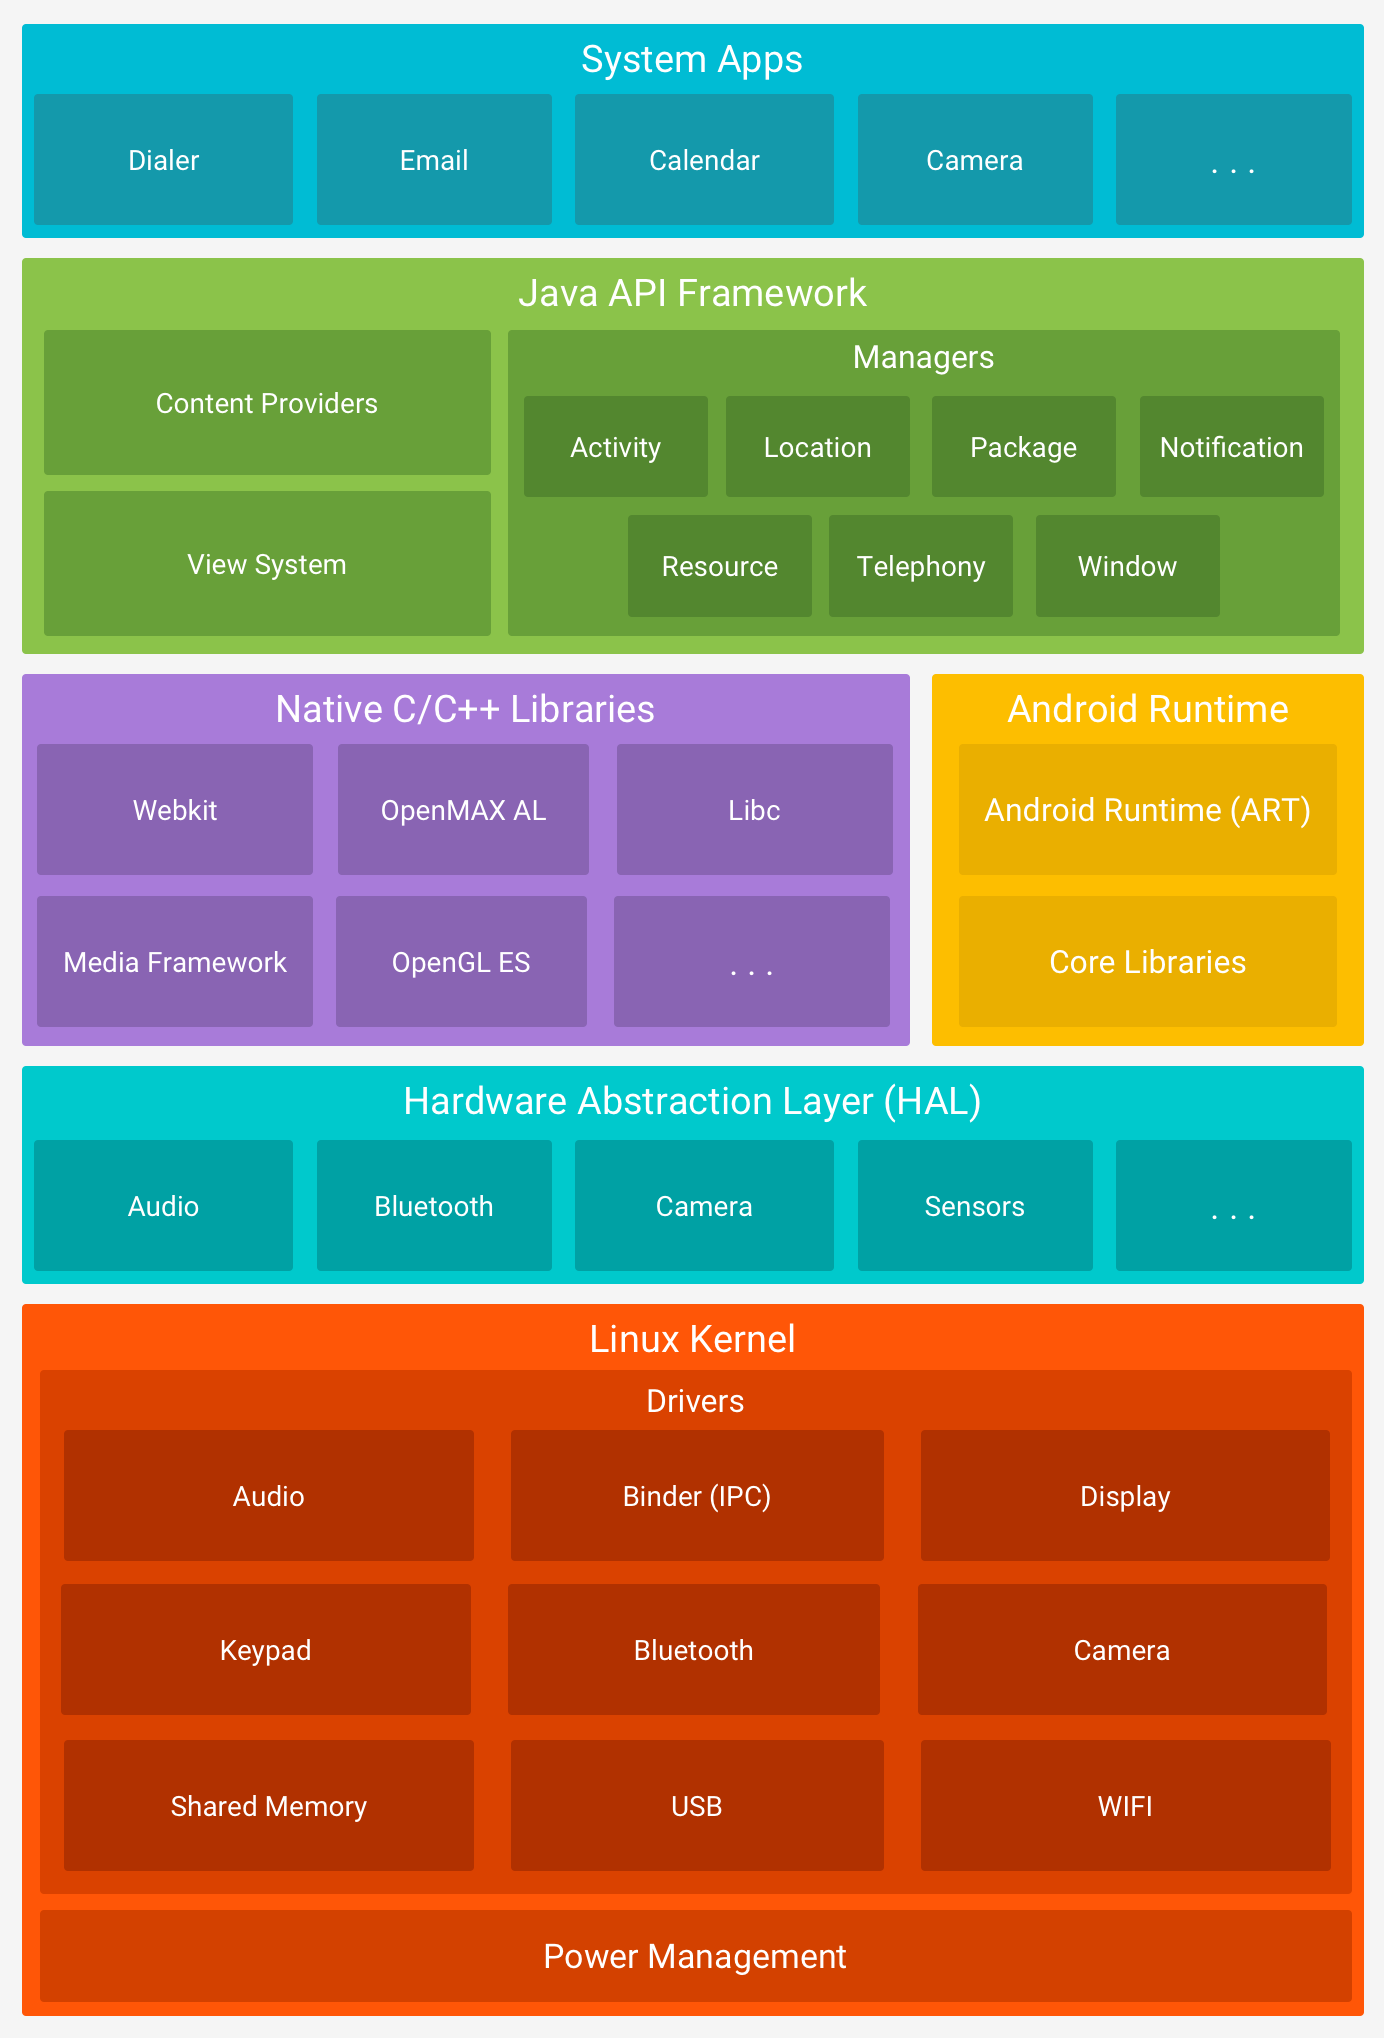
\includegraphics[width=0.9\textwidth, scale=0.9]{images/android}
	\caption{Android\label{fig:ALAP:sm2}}
\end{figure}

Az Android egy nyílt forráskódú, Linux kernel alapú többfelhasználós operációs rendszer, ahol minden applikáció egy külön felhasználó. Hivatalos nyelvei a Java és a Kotlin. Alapértelmezetten, a rendszer minden applikációnak kioszt egy egyedi Linux felhasználói ID-t (az ID-t csak a rendszer használja, és ismeretlen az applikáció számára). Az operációs rendszer úgy osztja ki a hozzáfárési jogokat az applikáció állományai számára, hogy csak az a felhasználói ID férjen hozzájuk, amivel az adott applikáció rendelkezik. Minden folyamat (process) rendelkezik a saját virtuális gépével, tehát minden applikáció kódja egymástól teljesen izoláltan fut. Alapértelmezetten minden applikáció a saját Linux folyamatában fut. Az Android operációs rendszer elindítja a folyamatot, amikor az applikáció valamelyik komponensének szüksége van rá, majd leállítja azt, mikor többé már nincs rá szükség, vagy ha a rendszernek mermóriát kell lefoglalnia, más applikációk számára. Az Android operációs rendszer “a legkevesebb kiváltság elvét” (“the principle of least privilige”) alkalmazza, tehát alapértelmezetten, minden applikációnak csak azokhoz a komponensekhez van hozzáférése, amik szükségesek a feladatának elvégzéséhez, és semmi egyébhez.

Egy android applikációnak négy fajta komponense lehet: Activity, Service, Broadcast receiver, Content provider. Ezek közül az Activity szolgál a felhasználóval történő interakció eszközéül, ez ugyanis egy felhasználói felülettel rendelkező képernyő. Activity-k, Service-k és Broadcast receiver-ek egy aszinkron üzenet által aktiválódnak, amit Intent-nek (szándék) nevezünk.

Az Activity egy osztály (class), amely a logikát tartalmazza, a felhasználói felületért azonban egy ehhez tartozó XML állomány felel, ami a különböző UI elemeket (gombok, szövegdobozok, konténerek) tartalmazza.

Az AndroidManifest.xml egy konfigurációs állomány, ami a projekt gyökér könyvtárában található. Itt vannak deklarálva az applikáció komponensei, valamint a szükséges hozzáférési jogokat is itt kell feltünteni.


%%%%%%%%%%%%%%%%%%%%%%%%%%%%%%%%%%%%%%%%%%%%%%%%%%%%%%%%%%%%%%%%%%%%%%%
\section{Gradle}\label{sec:ALAP:adatelem}

A Gradle egy nyílt forráskódú projektépítő eszköz (build automation tool). A Groovy, vagy Kotlin nyelvű scriptekbe, megadhatjuk a projektünk külső függöségeit (például API-k, library-k), melyeket letölti, majd lekompillálja és lefordítja a forráskódot.

\subsection{Teljesítmény}

\begin{description}
	\setlength{\itemsep}{0.04mm}
	\item[Inkrementális build] -- a Gradle leellenőrzi a build-ek futtatása között, hogy változtak-e a bemeneti adatok, a kimeneti adatok, vagy egy feladat implementációja az utolsó build meghívása óta. Ha nem változtak, akkor a feladatot (task) nem hajtja végre még egyszer. Egy faladat konfigurációja is bemeneti adatként tekintendő.
	\item[Inktrementális részfeladatok] -- részfeladatok esetén is számon tartja, hogy változtak-e a bemeneti, valamint a kimeneti adatok, így pontosan meg tudja állaptíani, hogy mi változott, így nem biztos, hogy mindent újra kell build-elnie.
	\item[Párhuzamos végrehajtás] -- lehetőség van a feladatok és a részfeladatok párhuzamos végrehajtására, ami jelentősen növeli a build végrehajtásának sebességét.
	\item[Függőségek párhuzamos letöltése] -- a függőségek letőltése párhuzamosan zajlik, igény szerint, vagyis csak akkor, amikor szükség van ezekre.
\end{description}

\subsection{Függőségkezelés}

\begin{description}
	\setlength{\itemsep}{0.04mm}
	\item[Tranzitív függőségek] -- függőség menedzselő rendszer lévén, a Gradle gondoskodik a tranzitív függőségek letöltéséről, valamint kezeléséről.
	\item[Külső függőségek] -- amikor a függőségek "távoli raktárakban" (remote repository) találhatóak, akkor ezeket eltárolja egy lokálisan, így egymást követő build-ek során újra felhasználja, elkerülvén a felesleges hálózati forgalmat.
\end{description}

\subsection{Android alkalmazások}

Az Andoid Studio-hoz (az android hivatalos fejlesztői környezete) tartozó Gradle kiegészítő az android alkalmazások hivatalos build eszköze, melyet az android fejlesztői csapata tart karban.

\begin{description}
	\setlength{\itemsep}{0.04mm}
	\item[Teljes integráció az Android Studio-val] -- a Gradle olyannyira mélyen van integrálva az Android Studio-ba, hogy az utóbbinak nincs is saját build eszköze, hanem őt bízza meg a build-elési feladatokkal.
	\item[Automatikus aláírás] -- automatikusan aláírja a fejlesztett applikációkat, ami szükséges ahhoz, hogy feltöltsük ezeket a Google Play áruházba.
	\item[Multidex támogatás] -- ez lehetővé teszi, hogy meghaladjuk a 65000-es metódusszám limitet, mely az Anroid DEX állományokra vonatkozik és az applikáció .apk-ba való csomagolásakor történik az ellenőrzése.
\end{description}

%%%%%%%%%%%%%%%%%%%%%%%%%%%%%%%%%%%%%%%%%%%%%%%%%%%%%%%%%%%%%%%%%%%%%%%
\section{Firebase}\label{sec:ALAP:szerkeszt}

A felhasználók adatainak, beállításainak tárolására, kezelésére a Firestore nevű no-sql (.json) alapú adatbázist használtam, mely a CRUD%
\footnote{ %
	create, read, update, delete
}  %
 műveletekhez is biztosít metódusokat. Logikai éptőelemei a kollekciók (collection) és a dokumentumok (document). Az előbbi tartalmazhat dokumentumokat, míg az utóbbi alkollekciókat, vagy magukat az adatokat. Az adatok kulcs, érték párok, az értékek lehetnek számok, karakterláncok, tömbök, geopontok vagy akár sajátos osztályok. Amennyiben sajátos osztály akarunk használni, annak rendelkeznie kell egy publikus konstruktorral, melynek nincsenek paraméterei, valamint az attribútumokhoz kell tartozzon egy-egy publikus „getter”%
 \footnote{ %
 	egy paraméter nélküli metódus, mely egy attribútumot térít vissza - példa: String getName()
 }  %
 metódus. Az adatbázisban található adatokhoz való hozzáférést egy szabállyal kell megadni, amelyet a szerver leellenőriz a CRUD műveletek végrehajtása esetén.

A felhasználók menedzselésére, mint a regisztráció, bejelentkezés, e-mail cím aktiválása, elfelejtett jelszó visszaállítása, a Firebase Authentication szolgáltatást használtam.

\subsection{Autentikáció}

\subsection{Firestore}


%%%%%%%%%%%%%%%%%%%%%%%%%%%%%%%%%%%%%%%%%%%%%%%%%%%%%%%%%%%%%%%%%%%%%%%
\section{Térkép}\label{sec:ALAP:szerkeszt}

\subsection{Distance Matrix API}



\subsection{Directions API}

A csomópontok közti távolságok mátrixának lekérdezésére a Distance Matrix API-t, valamint két csomópont közötti útvonal meghatározására a Directions API-t használtam.


